\documentclass[12pt]{article}
\usepackage[margin=1in]{geometry}
\usepackage{amsmath,amssymb,mathtools}
\usepackage{enumitem}
\usepackage{bm}
\usepackage{hyperref}
\usepackage{fancyhdr}
\usepackage{draftwatermark}
\usepackage{xcolor}
\usepackage{pgfplots}
\usepackage{titlesec}
\pgfplotsset{compat=newest}

%------------- TITLE AND METADATA -------------
\newcommand{\CourseCode}{HE2002 }
\newcommand{\CourseName}{Macroeconomics II}
\newcommand{\DocType}{Tutorial 6}

\title{
\CourseCode \CourseName \\[0.3em]
\large \DocType
}
\author{
  Academic Year 2025/2026, Semester 2 \\[0.25em]
  \textit{Quantitative Research Society @NTU}
}
\date{\today}

%------------- HEADER & FOOTER (for page 2 onward) -------------
\fancypagestyle{main}{
  \fancyhf{}
  \fancyhead[L]{\CourseCode \CourseName \ --\ \DocType}
  \fancyhead[R]{\href{https://qrsntu.org}{QRS@NTU}}
  \fancyfoot[C]{\thepage}
  \renewcommand{\headrulewidth}{0.4pt}
  \renewcommand{\footrulewidth}{0pt}
}

%------------- SIMPLE FOOTER (page 1 only) -------------
\fancypagestyle{plainfirst}{
  \fancyhf{}
  \renewcommand{\headrulewidth}{0pt}
  \renewcommand{\footrulewidth}{0pt}
  \fancyfoot[C]{\scriptsize\textcolor{gray}{\textit{For academic reference only. This document is provided for educational purposes and does not constitute an official question paper, answer key, or any formally authorised academic material. Its content is not guaranteed to be complete or accurate.}}}
}

%------------- WATERMARK -------------
\SetWatermarkText{Unofficial — QRS@NTU — qrsntu.org}
\SetWatermarkScale{1}
\SetWatermarkLightness{0.99}

%------------- SHORTCUTS -------------
\newcommand{\R}{\mathbb{R}}
\newcommand{\Rp}{\mathbb{R}_+}
\newcommand{\E}{\mathbb{E}}
\newcommand{\Var}{\mathrm{Var}}
\newcommand{\dotp}{\cdot}

%------------- STYLE -------------
\setlist[enumerate]{itemsep=0.32em, topsep=0.32em}
\setlist[itemize]{itemsep=0.22em, topsep=0.22em}

\titleformat{\subsubsection}[block]
{\normalfont\large\bfseries}
{}
{0pt}
{}

\titleformat{\paragraph}[block]
{\normalfont\normalsize\bfseries}
{}
{0pt}
{}

\titlespacing*{\paragraph}
{0pt}
{1.2ex}
{0.6ex}

\setcounter{secnumdepth}{0}
\setcounter{tocdepth}{4}

\begin{document}

\maketitle
\thispagestyle{plainfirst}
\pagestyle{main}
\bigskip

%====================================================
% OVERVIEW
%====================================================
\begin{center}
  \rule{0.8\textwidth}{0.4pt}\\[4pt]
  \textbf{Overview}\\[2pt]
  \rule{0.8\textwidth}{0.4pt}
\end{center}

\noindent
This tutorial covers:
\begin{itemize}[leftmargin=*]
  \item the wage-setting and price-setting framework in the labour market;
  \item the determination of the real wage under imperfect competition;
  \item the natural rate of unemployment and its dependence on the mark-up;
  \item the economic logic behind downward-sloping wage-setting relations;
  \item graphical and algebraic interpretations of equilibrium unemployment.
\end{itemize}

\bigskip

\newpage
\tableofcontents

\newpage
%====================================================
% QUESTION 1
%====================================================
\section{Question 1: The Natural Rate of Unemployment}

\noindent
Chapter 7, Q3. The natural rate of unemployment

\subsection{Problem}
Suppose that the markup of goods prices over marginal cost is 5\%, and that the wage-setting equation is
\[
W = P(1-u)
\]
where \(u\) is the unemployment rate.
\begin{enumerate}[label=(\alph*)]
    \item What is the real wage, as determined by the price-setting equation?
    \item What is the natural rate of unemployment?
    \item Suppose that the markup of prices over costs increases to 10\%. What happens to the natural rate of unemployment? Explain the logic behind your answer.
\end{enumerate}

\subsection{Solution}

\subsubsection{Method 1: Direct use of the WS--PS equations}
\begin{enumerate}[label=(\alph*)]
    \item
    Under price setting with mark-up \(m\), the standard relation is
    \[
    P=(1+m)W.
    \]
    Rearranging gives the real wage implied by firms' price setting:
    \[
    \frac{W}{P}=\frac{1}{1+m}.
    \]
    Here \(m=0.05\), so
    \[
    \frac{W}{P}=\frac{1}{1.05}=\frac{100}{105}=\frac{20}{21}\approx 0.9524.
    \]
    Hence the real wage determined by the price-setting equation is
    \[
    \boxed{\frac{W}{P}=\frac{20}{21}\approx 0.9524.}
    \]

    \item
    From the wage-setting equation,
    \[
    W=P(1-u),
    \]
    so dividing both sides by \(P\) gives
    \[
    \frac{W}{P}=1-u.
    \]
    At the natural rate of unemployment \(u_n\), the real wage implied by wage setting must equal the real wage implied by price setting. Therefore
    \[
    1-u_n=\frac{20}{21}.
    \]
    Hence
    \[
    u_n=1-\frac{20}{21}=\frac{1}{21}\approx 0.0476.
    \]
    Therefore the natural rate of unemployment is
    \[
    \boxed{u_n=\frac{1}{21}\approx 4.76\%.}
    \]

    \item
    If the mark-up increases to \(10\%\), then \(m=0.10\). The price-setting real wage becomes
    \[
    \frac{W}{P}=\frac{1}{1.10}=\frac{10}{11}\approx 0.9091.
    \]
    The natural rate is therefore determined by
    \[
    1-u_n=\frac{10}{11},
    \]
    so
    \[
    u_n=1-\frac{10}{11}=\frac{1}{11}\approx 0.0909.
    \]
    Thus the new natural rate of unemployment is
    \[
    \boxed{u_n=\frac{1}{11}\approx 9.09\%.}
    \]

    Comparing with part (b),
    \[
    \frac{1}{11}-\frac{1}{21}=\frac{10}{231}\approx 0.0433,
    \]
    so the natural rate rises by about \(4.33\) percentage points.

    The logic is as follows. A higher mark-up means firms set a higher price relative to wages. Equivalently, firms are willing to pay a lower real wage:
    \[
    \frac{W}{P}=\frac{1}{1+m}.
    \]
    To make workers accept this lower real wage, unemployment must be higher, because higher unemployment weakens workers' bargaining power and lowers the wage they seek. Hence the equilibrium natural rate of unemployment increases.
\end{enumerate}

\subsubsection{Method 2: WS--PS diagram and equilibrium intersection}
The labour-market equilibrium can be read from the intersection of:
\begin{itemize}[leftmargin=*]
    \item the wage-setting relation
    \[
    \frac{W}{P}=1-u,
    \]
    which is downward sloping in \(u\); and
    \item the price-setting relation
    \[
    \frac{W}{P}=\frac{1}{1+m},
    \]
    which is horizontal for any fixed \(m\).
\end{itemize}

\begin{center}
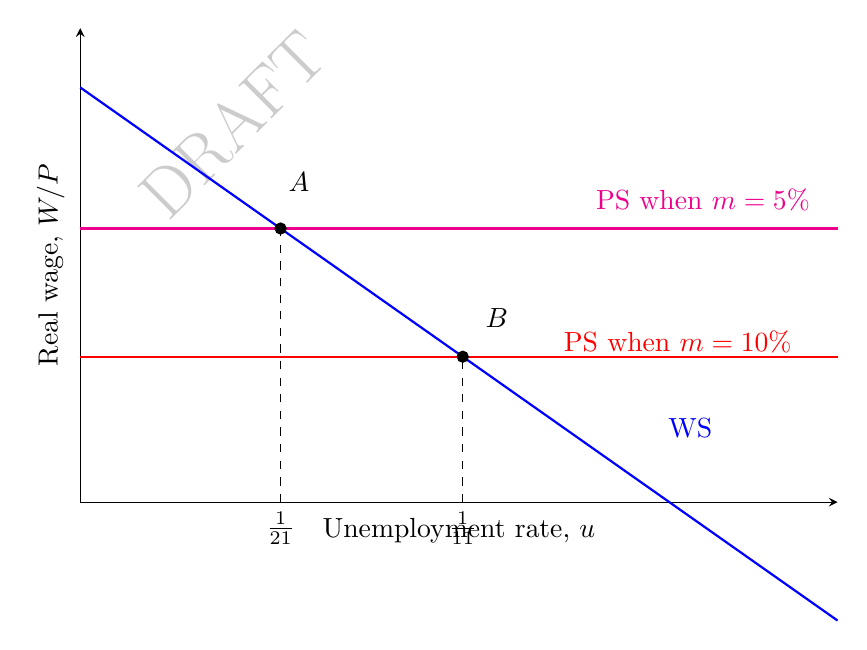
\begin{tikzpicture}
\begin{axis}[
    width=11.2cm,
    height=7.6cm,
    xmin=0,
    xmax=0.18,
    ymin=0.86,
    ymax=1.02,
    axis lines=left,
    xlabel={Unemployment rate, \(u\)},
    ylabel={Real wage, \(W/P\)},
    xtick=\empty,
    ytick=\empty,
    clip=false
]
\addplot[domain=0:0.18,samples=2,thick,blue] {1-x};
\addplot[domain=0:0.18,samples=2,thick,magenta] {20/21};
\addplot[domain=0:0.18,samples=2,thick,red] {10/11};

\addplot[dashed] coordinates {(1/21,0.86) (1/21,20/21)};
\addplot[dashed] coordinates {(1/11,0.86) (1/11,10/11)};

\addplot[only marks,mark=*,mark size=2pt] coordinates {(1/21,20/21) (1/11,10/11)};

\node[blue] at (axis cs:0.145,0.885) {WS};
\node[magenta] at (axis cs:0.148,0.962) {PS when \(m=5\%\)};
\node[red] at (axis cs:0.142,0.914) {PS when \(m=10\%\)};
\node at (axis cs:0.052,0.968) {\(A\)};
\node at (axis cs:0.099,0.922) {\(B\)};
\node[anchor=north] at (axis cs:1/21,0.86) {\(\frac{1}{21}\)};
\node[anchor=north] at (axis cs:1/11,0.86) {\(\frac{1}{11}\)};
\end{axis}
\end{tikzpicture}
\end{center}

\begin{enumerate}[label=(\alph*)]
    \item
    For \(m=0.05\), the price-setting line is at height
    \[
    \frac{1}{1.05}=\frac{20}{21}.
    \]
    So the real wage is
    \[
    \boxed{\frac{W}{P}=\frac{20}{21}\approx 0.9524.}
    \]

    \item
    The natural rate is the unemployment rate at the intersection \(A\), where
    \[
    1-u_n=\frac{20}{21}.
    \]
    Therefore
    \[
    \boxed{u_n=\frac{1}{21}\approx 4.76\%.}
    \]

    \item
    When the mark-up increases to \(10\%\), the price-setting line shifts down from
    \[
    \frac{20}{21}
    \quad\text{to}\quad
    \frac{10}{11}.
    \]
    The new equilibrium is at \(B\), where
    \[
    1-u_n=\frac{10}{11}.
    \]
    Hence
    \[
    \boxed{u_n=\frac{1}{11}\approx 9.09\%.}
    \]
    So the natural rate of unemployment rises. Graphically, the lower PS line intersects the WS curve further to the right, which means a higher unemployment rate is required to reduce workers' wage demands enough to restore equilibrium.
\end{enumerate}

\newpage
%====================================================
% QUESTION 2
%====================================================
\section{Question 2: The Existence of Unemployment}

\noindent
Chapter 7, Q6. The existence of unemployment

\subsection{Problem}
\begin{enumerate}[label=(\alph*)]
    \item Why does the wage-setting relation in the Figure have a downward slope? As employment \(N\) approaches labor force \(L\), what happens to the unemployment rate?
    \item The price-setting relation is horizontal. How would an increase in the mark-up affect the position of the price-setting relation in the Figure? How would an increase in the mark-up affect the natural rate of unemployment in the Figure?
\end{enumerate}

\begin{center}
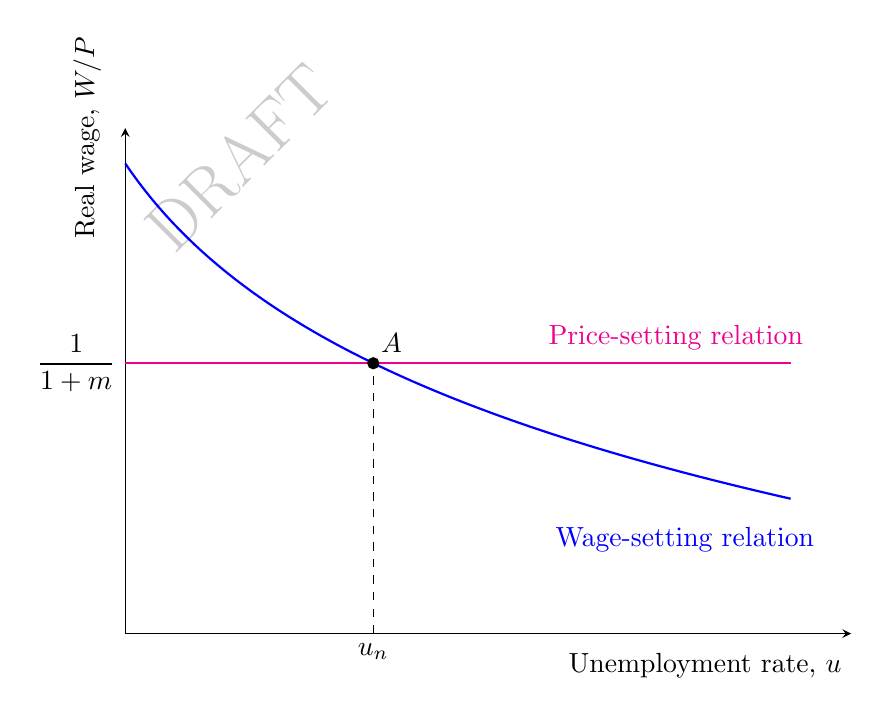
\begin{tikzpicture}
\begin{axis}[
    width=10.8cm,
    height=8cm,
    xmin=0,
    xmax=0.24,
    ymin=0.72,
    ymax=1.15,
    axis lines=left,
    xlabel={Unemployment rate, \(u\)},
    ylabel={Real wage, \(W/P\)},
    % --- Added styles to move labels to the ends ---
    xlabel style={at={(axis description cs:1,-0.02)}, anchor=north east},
    ylabel style={at={(axis description cs:-0.02,1.2)}, anchor=south east},
    % -----------------------------------------------
    xtick=\empty,
    ytick=\empty,
    clip=false
]
\addplot[domain=0:0.22,samples=200,thick,blue] {1.12 - 0.1524*ln(1+25*x)};
\addplot[domain=0:0.22,samples=2,thick,magenta] {0.95};
\addplot[dashed] coordinates {(0.082,0.72) (0.082,0.95)};
\addplot[only marks,mark=*,mark size=2pt] coordinates {(0.082,0.95)};

\node[blue] at (axis cs:0.185,0.8) {Wage-setting relation};
\node[magenta] at (axis cs:0.182,0.972) {Price-setting relation};
\node at (axis cs:0.088,0.967) {\(A\)};
\node[anchor=east] at (axis cs:0,0.95) {\(\dfrac{1}{1+m}\)};
\node[anchor=north] at (axis cs:0.082,0.72) {\(u_n\)};
\end{axis}
\end{tikzpicture}
\end{center}


\newpage
\subsection{Solution}

\subsubsection{Method 1: Graph-first economic reasoning}
\begin{enumerate}[label=(\alph*)]
    \item
    The wage-setting relation is downward sloping because a higher unemployment rate weakens workers' bargaining power. When unemployment is high, workers are more afraid of job loss and unemployed workers compete more intensely for jobs, so firms can pay a lower real wage. When unemployment is low, workers have stronger bargaining power and wage claims are higher.

    Therefore, as \(u\) rises, the real wage consistent with wage setting falls, which is why the WS relation slopes downward.

    The unemployment rate is
    \[
    u=\frac{L-N}{L}=1-\frac{N}{L}.
    \]
    As employment \(N\) approaches labour force \(L\),
    \[
    \frac{N}{L}\to 1,
    \]
    so
    \[
    u=1-\frac{N}{L}\to 0.
    \]
    Hence, as employment approaches the labour force, the unemployment rate tends to zero:
    \[
    \boxed{u\to 0 \text{ as } N\to L.}
    \]

    \item
    The price-setting relation is horizontal because the real wage implied by firms' price setting is
    \[
    \frac{W}{P}=\frac{1}{1+m},
    \]
    which does not depend on \(u\). For any given mark-up \(m\), firms are willing to pay the same real wage regardless of the unemployment rate, so the PS line is flat.

    If the mark-up increases, then \(1/(1+m)\) falls. Therefore the PS line shifts downward.

    The natural rate of unemployment is determined by the intersection of WS and PS. If PS shifts downward while WS is unchanged, the new intersection occurs at a higher value of unemployment. Thus the natural rate of unemployment rises.

    So the answer is:
    \[
    \boxed{\text{A higher mark-up shifts PS downward and increases }u_n.}
    \]
\end{enumerate}

\subsubsection{Method 2: Formal algebra using the general equilibrium condition}
Let the wage-setting relation be written more generally as
\[
\frac{W}{P}=F(u),
\]
where
\[
F'(u)<0.
\]
This captures the idea that the real wage demanded by workers is lower when unemployment is higher.

The price-setting relation is
\[
\frac{W}{P}=\frac{1}{1+m}.
\]
Equilibrium in the labour market therefore requires
\[
F(u_n)=\frac{1}{1+m}.
\]

\begin{enumerate}[label=(\alph*)]
    \item
    Since \(F'(u)<0\), the wage-setting relation is downward sloping in \(u\). This is the formal version of the claim that higher unemployment reduces wage pressure.

    Also,
    \[
    u=\frac{L-N}{L}=1-\frac{N}{L}.
    \]
    Hence if \(N\to L\), then
    \[
    \frac{N}{L}\to 1
    \quad\Longrightarrow\quad
    u\to 0.
    \]
    Therefore
    \[
    \boxed{u\to 0 \text{ as } N\to L.}
    \]

    \item
    The PS relation is horizontal because its height is determined solely by \(m\):
    \[
    \omega_{PS}(m):=\frac{1}{1+m}.
    \]
    Differentiating with respect to \(m\),
    \[
    \omega_{PS}'(m)=-\frac{1}{(1+m)^2}<0.
    \]
    So a higher mark-up lowers the real wage consistent with price setting; graphically, PS shifts downward.

    To determine the effect on the natural rate, differentiate the equilibrium condition
    \[
    F(u_n)=\frac{1}{1+m}
    \]
    with respect to \(m\):
    \[
    F'(u_n)\frac{du_n}{dm}=-\frac{1}{(1+m)^2}.
    \]
    Therefore
    \[
    \frac{du_n}{dm}
    =
    \frac{-1/(1+m)^2}{F'(u_n)}.
    \]
    Since \(F'(u_n)<0\), the denominator is negative, while the numerator is also negative, so
    \[
    \frac{du_n}{dm}>0.
    \]
    Thus an increase in the mark-up raises the natural rate of unemployment:
    \[
    \boxed{\frac{du_n}{dm}>0 \quad\Longrightarrow\quad \text{a higher mark-up increases }u_n.}
    \]
\end{enumerate}

\end{document}